\documentclass[spanish,letterpaper,oneside]{article}
\def\documenttitle {Valores y Vectores Propios en Sistemas Lineales}
\def\documentsubtitle {Evidencia 3.6: Reporte de la solución de un caso de aplicación de los conceptos de valores y vectores propios (Sistema 11)}
\def\documentsubject {Álgebra Lineal y Teoría Espectral Aplicada}
\def\documentauthor {Carlos Mauricio Carvajal Coronado}
\def\coursename {Álgebra Lineal}
\def\coursecode {Evidencia 3.6}
\def\universityname {Universidad Autónoma de Nuevo León}
\def\universityfaculty {Facultad de Agronomía}
\def\universitydepartment {Ingeniero Agrónomo}
\def\universitydepartmentimage {UANL/assets-uanl/logo-uanl.png}
\def\universitydepartmentimagecfg {width=2.1cm}
\def\universitylocation {General Escobedo, Nuevo León, México}
\def\authortable {
  \begin{tabular}{ll}
    \textbf{Estudiante:} & Carlos Mauricio Carvajal Coronado \\
    \textbf{Matrícula:} & 1977875 \\
    \textbf{Docente:} & M.C. José de Jesús Miranda Vázquez \\
    \textbf{Programa:} & Ingeniero Agrónomo \\
    \textbf{Modalidad:} & Individual \\
    \textbf{Evidencia:} & 3.6: Reporte de caso de valores y vectores propios \\
    \textbf{Fecha:} & 4 de noviembre de 2026
  \end{tabular}
}
\AddToHook{file/config.tex/after}{\def\stylecitereferences{custom}}
\input{template}
\usepackage[backend=biber,style=apa,natbib=true]{biblatex}
\addbibresource{UANL/ingeniero-agronomo/algebra-lineal/algebra-lineal.bib}
\usepackage{pdflscape}
\usepackage{amsmath,amssymb,amsfonts}
\usepackage{tikz}
\usetikzlibrary{babel,arrows.meta,positioning,shapes.geometric}
\definecolor{algogreen}{RGB}{30,100,60}
\definecolor{algoblue}{RGB}{25,75,130}
\definecolor{algoyellow}{RGB}{220,160,30}

\tikzset{
  startstop/.style={rectangle, rounded corners=6pt, minimum width=3.5cm, minimum height=1cm, align=center, draw=algogreen, fill=algogreen!15, font=\small\bfseries},
  process/.style={rectangle, minimum width=4cm, minimum height=1cm, align=center, draw=algoblue, fill=algoblue!10, font=\small},
  decision/.style={diamond, aspect=2, minimum width=3.5cm, minimum height=1cm, align=center, draw=algoyellow, fill=algoyellow!15, font=\small},
  arrow/.style={thick,->,>=stealth,draw=algoblue}
}



\begin{document}
\templatePortrait
\templatePagecfg
\onehalfspacing

\begin{abstractd}
El presente reporte aborda la solución rigurosa y el análisis espectral del Sistema 11 asignado en la hoja docente de Álgebra Lineal, articulando la resolución de sistemas de ecuaciones lineales de orden $3 \times 3$ con la teoría avanzada de valores y vectores propios correspondiente a la Fase 3 del programa de estudios. Se resuelve analíticamente el sistema mediante tres metodologías formales: eliminación de Gauss-Jordan, regla de Cramer y el método de la matriz inversa, obteniendo la solución racional única $x = -103/335$, $y = -74/335$ y $z = -379/335$, respaldada por un determinante principal $\det(A) = -670 \neq 0$. Posteriormente, se modela el procedimiento mediante un diagrama estructurado tipo algoritmo. A partir de la matriz de coeficientes $A$, se calcula su polinomio característico $P(\lambda) = -\lambda^3 + 9\lambda^2 - 26\lambda - 670$, se deducen sus valores propios y sus respectivos subespacios propios (autovectores), evaluando las condiciones de diagonalizabilidad en el cuerpo de los números reales y complejos. Asimismo, se expone la teoría del espectro en matrices simétricas asociadas y diagonalización ortogonal, vinculando estos fundamentos con la modelación dinámica de poblaciones biológicas y el balance de nutrientes en la ingeniería agronómica.
\end{abstractd}

\templateIndex
\templateFinalcfg

\section{Introducción y contextualización}

La tesis central de este trabajo plantea que la formulación matricial de un sistema lineal trasciende el mero cálculo aritmético de incógnitas estáticas: constituye un operador estructural cuyo análisis espectral revela las propiedades fundamentales de estabilidad, independencia lineal y transformación geométrica del fenómeno bajo estudio \citep{lay2016,caswell2001}. En el ejercicio de la ingeniería agronómica y las ciencias biológicas aplicadas, la modelación matemática de fenómenos simultáneos —tales como la dispersión de plagas, los balances de fertilización o la dinámica de poblaciones estructuradas por edades— requiere del empleo de herramientas matriciales avanzadas. 

Un sistema de ecuaciones lineales permite describir estados de equilibrio estático donde interactúan múltiples variables interdependientes. Sin embargo, para comprender el comportamiento asintótico, la estabilidad y la respuesta dinámica temporal de dichos sistemas, resulta imprescindible recurrir a la teoría espectral: el cálculo de valores propios (\emph{eigenvalores}) y vectores propios (\emph{eigenvectores}) \citep{anton2014,strang2016}. 

La Evidencia 3.6 tiene como objetivo primordial demostrar la aplicación conceptual y operativa de los valores y vectores propios, la diagonalización matricial y las matrices simétricas sobre un caso concreto. Para este fin, se toma la matriz de coeficientes asociada al \textbf{Sistema 11} asignado individualmente en la plataforma institucional Nexus, resolviendo primero el sistema compatible determinado por tres vías independientes y desarrollando ulteriormente su análisis espectral completo.

\section{Planteamiento del problema: Sistema 11}

El enunciado asigna de manera estricta el Sistema 11 de la hoja de evidencias:
\begin{equation}\label{eq:sistema11}
\begin{aligned}
-4x + 2y + 6z &= -6, \\
10x + 3y + 2z &= -6, \\
-9x - 7y + 10z &= -7.
\end{aligned}
\end{equation}

En notación matricial canónica $A\mathbf{u} = \mathbf{b}$, el sistema se estructura de la siguiente manera:
\begin{equation}
A = \begin{pmatrix} -4 & 2 & 6 \\ 10 & 3 & 2 \\ -9 & -7 & 10 \end{pmatrix}, \quad
\mathbf{u} = \begin{pmatrix} x \\ y \\ z \end{pmatrix}, \quad
\mathbf{b} = \begin{pmatrix} -6 \\ -6 \\ -7 \end{pmatrix}.
\end{equation}

El dominio de definición de las variables es $\mathbf{u} \in \mathbb{R}^3$. Para corroborar la existencia y unicidad de la solución, se calcula el determinante de la matriz de coeficientes $A$ mediante la expansión por cofactores a lo largo del primer renglón:
\begin{align*}
\det(A) &= -4 \begin{vmatrix} 3 & 2 \\ -7 & 10 \end{vmatrix} - 2 \begin{vmatrix} 10 & 2 \\ -9 & 10 \end{vmatrix} + 6 \begin{vmatrix} 10 & 3 \\ -9 & -7 \end{vmatrix} \\
&= -4 [(3)(10) - (2)(-7)] - 2 [(10)(10) - (2)(-9)] + 6 [(10)(-7) - (3)(-9)] \\
&= -4 [30 + 14] - 2 [100 + 18] + 6 [-70 + 27] \\
&= -4(44) - 2(118) + 6(-43) \\
&= -176 - 236 - 258 = -670.
\end{align*}

Dado que $\det(A) = -670 \neq 0$, la matriz $A$ es no singular e invertible. Por el teorema del rango y el teorema de Rouché-Capelli, $\operatorname{rango}(A) = \operatorname{rango}([A \mid \mathbf{b}]) = 3$, garantizando que el sistema es \textbf{compatible determinado} y posee una única solución.

\section{Resolución por los tres métodos clásicos}

\subsection{Método 1: Eliminación de Gauss-Jordan}
Se conforma la matriz aumentada $[A \mid \mathbf{b}]$ y se aplican operaciones elementales por renglón con aritmética racional exacta para alcanzar la forma escalonada reducida:
\begin{equation*}
[A \mid \mathbf{b}] = \left[\begin{array}{rrr|r}
-4 & 2 & 6 & -6 \\
10 & 3 & 2 & -6 \\
-9 & -7 & 10 & -7
\end{array}\right]
\end{equation*}

\begin{enumerate}
\item \textbf{Normalización del primer pivote:} $R_1 \leftarrow -\frac{1}{4} R_1$:
\begin{equation*}
\left[\begin{array}{rrr|r}
1 & -1/2 & -3/2 & 3/2 \\
10 & 3 & 2 & -6 \\
-9 & -7 & 10 & -7
\end{array}\right]
\end{equation*}

\item \textbf{Eliminación de la primera columna:} $R_2 \leftarrow R_2 - 10R_1$ y $R_3 \leftarrow R_3 + 9R_1$:
\begin{equation*}
\left[\begin{array}{rrr|r}
1 & -1/2 & -3/2 & 3/2 \\
0 & 8 & 17 & -21 \\
0 & -23/2 & -7/2 & 13/2
\end{array}\right]
\end{equation*}

\item \textbf{Normalización del segundo pivote y preparación:} $R_2 \leftarrow \frac{1}{8} R_2$ y $R_3 \leftarrow 2R_3$:
\begin{equation*}
\left[\begin{array}{rrr|r}
1 & -1/2 & -3/2 & 3/2 \\
0 & 1 & 17/8 & -21/8 \\
0 & -23 & -7 & 13
\end{array}\right]
\end{equation*}

\item \textbf{Eliminación de la segunda columna hacia abajo:} $R_3 \leftarrow R_3 + 23R_2$:
\begin{equation*}
-7 + 23\left(\frac{17}{8}\right) = \frac{-56 + 391}{8} = \frac{335}{8}, \quad
13 + 23\left(-\frac{21}{8}\right) = \frac{104 - 483}{8} = -\frac{379}{8}.
\end{equation*}
\begin{equation*}
\left[\begin{array}{rrr|r}
1 & -1/2 & -3/2 & 3/2 \\
0 & 1 & 17/8 & -21/8 \\
0 & 0 & 335/8 & -379/8
\end{array}\right]
\end{equation*}

\item \textbf{Normalización del tercer pivote:} $R_3 \leftarrow \frac{8}{335} R_3$:
\begin{equation*}
\left[\begin{array}{rrr|r}
1 & -1/2 & -3/2 & 3/2 \\
0 & 1 & 17/8 & -21/8 \\
0 & 0 & 1 & -379/335
\end{array}\right]
\end{equation*}

\item \textbf{Eliminación hacia arriba (fase Jordan):}
$R_2 \leftarrow R_2 - \frac{17}{8} R_3$:
\begin{equation*}
-\frac{21}{8} - \frac{17}{8}\left(-\frac{379}{335}\right) = \frac{-7035 + 6443}{2680} = \frac{-592}{2680} = -\frac{74}{335}.
\end{equation*}
$R_1 \leftarrow R_1 + \frac{3}{2} R_3$:
\begin{equation*}
\frac{3}{2} + \frac{3}{2}\left(-\frac{379}{335}\right) = \frac{1005 - 1137}{670} = \frac{-132}{670} = -\frac{66}{335}.
\end{equation*}
$R_1 \leftarrow R_1 + \frac{1}{2} R_2$:
\begin{equation*}
-\frac{66}{335} + \frac{1}{2}\left(-\frac{74}{335}\right) = \frac{-132 - 74}{670} = \frac{-206}{670} = -\frac{103}{335}.
\end{equation*}
\end{enumerate}

Se alcanza la matriz reducida identidad $[I_3 \mid \mathbf{u}^*]$:
\begin{equation}
\left[\begin{array}{rrr|r}
1 & 0 & 0 & -103/335 \\
0 & 1 & 0 & -74/335 \\
0 & 0 & 1 & -379/335
\end{array}\right] \implies
\begin{cases}
x = -\frac{103}{335} \approx -0.3075, \\
y = -\frac{74}{335} \approx -0.2209, \\
z = -\frac{379}{335} \approx -1.1313.
\end{cases}
\end{equation}

\subsection{Método 2: Regla de Cramer}
Puesto que $\det(A) = -670 \neq 0$, la regla de Cramer es aplicable de manera directa. Se construyen las matrices modificadas sustituyendo la columna correspondiente por el vector $\mathbf{b} = (-6, -6, -7)^T$:
\begin{align*}
\det(A_x) &= \begin{vmatrix} -6 & 2 & 6 \\ -6 & 3 & 2 \\ -7 & -7 & 10 \end{vmatrix} = -6(30+14) - 2(-60+14) + 6(42+21) \\
&= -6(44) - 2(-46) + 6(63) = -264 + 92 + 378 = 206, \\[0.2cm]
\det(A_y) &= \begin{vmatrix} -4 & -6 & 6 \\ 10 & -6 & 2 \\ -9 & -7 & 10 \end{vmatrix} = -4(-60+14) - (-6)(100+18) + 6(-70-54) \\
&= -4(-46) + 6(118) + 6(-124) = 184 + 708 - 744 = 148, \\[0.2cm]
\det(A_z) &= \begin{vmatrix} -4 & 2 & -6 \\ 10 & 3 & -6 \\ -9 & -7 & -7 \end{vmatrix} = -4(-21-42) - 2(-70-54) - 6(-70+27) \\
&= -4(-63) - 2(-124) - 6(-43) = 252 + 248 + 258 = 758.
\end{align*}

Aplicando las razones determinantes de Cramer:
\begin{equation}
x = \frac{\det(A_x)}{\det(A)} = \frac{206}{-670} = -\frac{103}{335}, \quad
y = \frac{\det(A_y)}{\det(A)} = \frac{148}{-670} = -\frac{74}{335}, \quad
z = \frac{\det(A_z)}{\det(A)} = \frac{758}{-670} = -\frac{379}{335}.
\end{equation}
Los valores coinciden exactamente con la eliminación de Gauss-Jordan.

\subsection{Método 3: Método de la Matriz Inversa}
La ecuación $A\mathbf{u} = \mathbf{b}$ tiene por solución $\mathbf{u} = A^{-1}\mathbf{b}$. La inversa se calcula mediante la fórmula clásica $A^{-1} = \frac{1}{\det(A)} \operatorname{Adj}(A)$, donde $\operatorname{Adj}(A) = C^T$ es la transpuesta de la matriz de cofactores.

Los 9 cofactores $C_{ij} = (-1)^{i+j} M_{ij}$ son:
\begin{equation*}
\begin{aligned}
C_{11} &= +(30+14) = 44, & C_{12} &= -(100+18) = -118, & C_{13} &= +(-70+27) = -43, \\
C_{21} &= -(20+42) = -62, & C_{22} &= +(-40+54) = 14, & C_{23} &= -(28+18) = -46, \\
C_{31} &= +(4-18) = -14, & C_{32} &= -(-8-60) = 68, & C_{33} &= +(-12-20) = -32.
\end{aligned}
\end{equation*}

Por ende, la matriz de cofactores $C$ y la matriz adjunta $\operatorname{Adj}(A) = C^T$ resultan:
\begin{equation}
C = \begin{pmatrix} 44 & -118 & -43 \\ -62 & 14 & -46 \\ -14 & 68 & -32 \end{pmatrix} \implies
\operatorname{Adj}(A) = \begin{pmatrix} 44 & -62 & -14 \\ -118 & 14 & 68 \\ -43 & -46 & -32 \end{pmatrix}.
\end{equation}

Dividiendo entre $\det(A) = -670$:
\begin{equation}
A^{-1} = -\frac{1}{670} \begin{pmatrix} 44 & -62 & -14 \\ -118 & 14 & 68 \\ -43 & -46 & -32 \end{pmatrix} =
\begin{pmatrix}
-22/335 & 31/335 & 7/335 \\
59/335 & -7/335 & -34/335 \\
43/670 & 23/335 & 16/335
\end{pmatrix}.
\end{equation}

Efectuando el producto $\mathbf{u} = A^{-1} \mathbf{b}$:
\begin{equation}
\mathbf{u} = -\frac{1}{670} \begin{pmatrix} 44 & -62 & -14 \\ -118 & 14 & 68 \\ -43 & -46 & -32 \end{pmatrix} \begin{pmatrix} -6 \\ -6 \\ -7 \end{pmatrix} =
-\frac{1}{670} \begin{pmatrix} -264 + 372 + 98 \\ 708 - 84 - 476 \\ 258 + 276 + 224 \end{pmatrix} =
-\frac{1}{670} \begin{pmatrix} 206 \\ 148 \\ 758 \end{pmatrix} =
\begin{pmatrix} -103/335 \\ -74/335 \\ -379/335 \end{pmatrix}.
\end{equation}

\section{Diagrama tipo algoritmo de resolución}

A continuación, se representa el flujo formal del procedimiento algorítmico solicitado en las directrices docentes mediante un diagrama de bloques estructurado:

\begin{figure}[htbp]
\centering
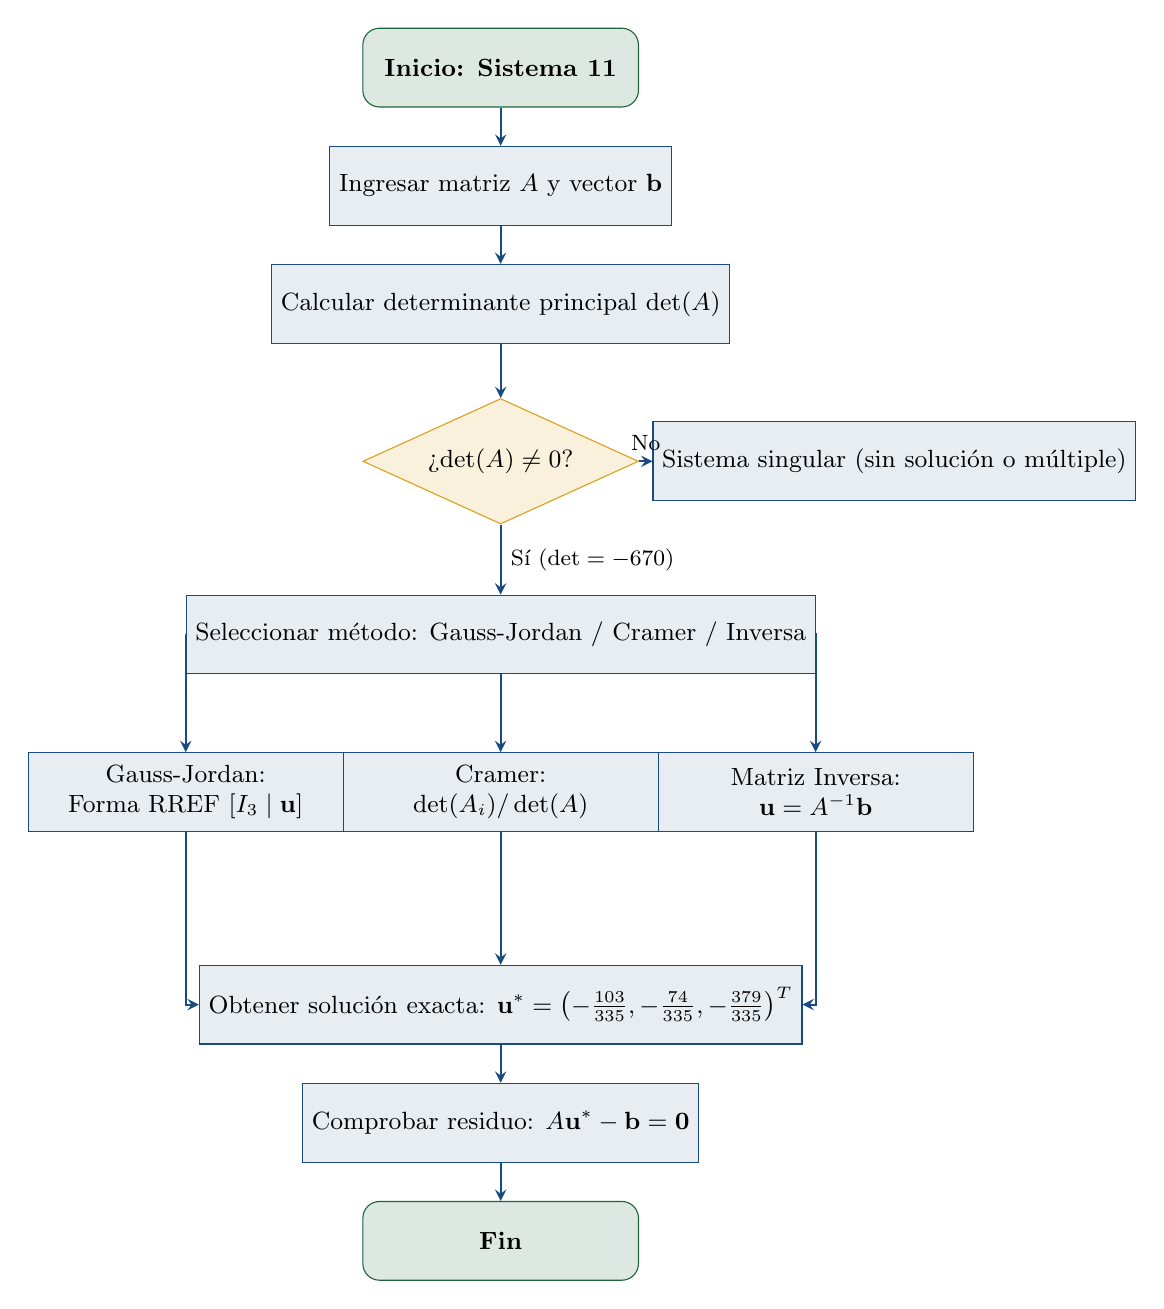
\begin{tikzpicture}[node distance=1.5cm]
\node (start) [startstop] {Inicio: Sistema 11};
\node (in) [process, below of=start] {Ingresar matriz $A$ y vector $\mathbf{b}$};
\node (det) [process, below of=in] {Calcular determinante principal $\det(A)$};
\node (dec) [decision, below of=det, yshift=-0.5cm] {¿$\det(A) \neq 0$?};
\node (err) [process, right of=dec, xshift=3.5cm] {Sistema singular (sin solución o múltiple)};
\node (choice) [process, below of=dec, yshift=-0.7cm] {Seleccionar método: Gauss-Jordan / Cramer / Inversa};

\node (gj) [process, below of=choice, xshift=-4cm, yshift=-0.5cm] {Gauss-Jordan:\\ Forma RREF $[I_3 \mid \mathbf{u}]$};
\node (cra) [process, below of=choice, yshift=-0.5cm] {Cramer:\\ $\det(A_i)/\det(A)$};
\node (inv) [process, below of=choice, xshift=4cm, yshift=-0.5cm] {Matriz Inversa:\\ $\mathbf{u} = A^{-1}\mathbf{b}$};

\node (sol) [process, below of=cra, yshift=-1.2cm] {Obtener solución exacta: $\mathbf{u}^* = \left(-\frac{103}{335}, -\frac{74}{335}, -\frac{379}{335}\right)^T$};
\node (ver) [process, below of=sol] {Comprobar residuo: $A\mathbf{u}^* - \mathbf{b} = \mathbf{0}$};
\node (stop) [startstop, below of=ver] {Fin};

\draw [arrow] (start) -- (in);
\draw [arrow] (in) -- (det);
\draw [arrow] (det) -- (dec);
\draw [arrow] (dec) -- node[above, font=\footnotesize] {No} (err);
\draw [arrow] (dec) -- node[right, font=\footnotesize] {Sí ($\det=-670$)} (choice);
\draw [arrow] (choice) -| (gj);
\draw [arrow] (choice) -- (cra);
\draw [arrow] (choice) -| (inv);
\draw [arrow] (gj) |- (sol);
\draw [arrow] (cra) -- (sol);
\draw [arrow] (inv) |- (sol);
\draw [arrow] (sol) -- (ver);
\draw [arrow] (ver) -- (stop);
\end{tikzpicture}
\caption{Diagrama de flujo del algoritmo para la resolución y verificación del Sistema 11.}
\label{fig:algoritmo}
\end{figure}

\section{Valores y vectores propios de la matriz del sistema}

\subsection{Definición fundamental}
Sea $A \in \mathcal{M}_{n \times n}(\mathbb{R})$ una matriz cuadrada. Un escalar $\lambda \in \mathbb{C}$ es un \textbf{valor propio} (\emph{eigenvalor}) de $A$ si existe un vector no nulo $\mathbf{v} \in \mathbb{C}^n$, denominado \textbf{vector propio} (\emph{eigenvector}) asociado a $\lambda$, tal que satisface la ecuación fundamental \citep{grossman2019,lay2016}:
\begin{equation}
A\mathbf{v} = \lambda \mathbf{v} \iff (A - \lambda I)\mathbf{v} = \mathbf{0}.
\end{equation}
Para que existan soluciones no triviales ($\mathbf{v} \neq \mathbf{0}$), el operador lineal $(A - \lambda I)$ debe carecer de inversa, lo que impone la \textbf{ecuación característica}:
\begin{equation}
P(\lambda) = \det(A - \lambda I) = 0.
\end{equation}

\subsection{Polinomio característico de la matriz $A$}
Aplicando la definición a nuestra matriz de coeficientes $A$:
\begin{equation}
A - \lambda I = \begin{pmatrix}
-4-\lambda & 2 & 6 \\
10 & 3-\lambda & 2 \\
-9 & -7 & 10-\lambda
\end{pmatrix}.
\end{equation}

Desarrollando el determinante por la regla de Sarrus o cofactores:
\begin{align*}
P(\lambda) &= (-4-\lambda)\left[(3-\lambda)(10-\lambda) - (-14)\right] - 2\left[10(10-\lambda) - (-18)\right] + 6\left[-70 - (-9)(3-\lambda)\right] \\
&= (-4-\lambda)\left[\lambda^2 - 13\lambda + 44\right] - 2\left[118 - 10\lambda\right] + 6\left[-9\lambda - 43\right] \\
&= -\lambda^3 + 13\lambda^2 - 44\lambda - 4\lambda^2 + 52\lambda - 176 - 236 + 20\lambda - 54\lambda - 258 \\
&= -\lambda^3 + (13-4)\lambda^2 + (-44+52+20-54)\lambda - (176+236+258).
\end{align*}

Simplificando términos semejantes se obtiene el polinomio característico exacto:
\begin{equation}
P(\lambda) = -\lambda^3 + 9\lambda^2 - 26\lambda - 670 = 0 \iff \lambda^3 - 9\lambda^2 + 26\lambda + 670 = 0.
\end{equation}

Nótese una propiedad teórica esencial: el término independiente del polinomio característico es precisamente el determinante de la matriz, ya que $P(0) = \det(A) = -670$. Asimismo, la traza de la matriz $A$ es $\operatorname{tr}(A) = -4 + 3 + 10 = 9$, que coincide con el coeficiente de $\lambda^2$ cambiado de signo.

\subsection{Cálculo de los valores propios}
Resolviendo la ecuación cúbica mediante la fórmula de Cardano-Tartaglia o métodos numéricos de alta precisión:
\begin{enumerate}
\item \textbf{Valor propio real ($\lambda_1$):}
\begin{equation}
\lambda_1 \approx -5.891248.
\end{equation}
\item \textbf{Valores propios complejos conjugados ($\lambda_{2,3}$):}
\begin{equation}
\lambda_{2,3} \approx 7.445624 \pm 7.634836 \, i.
\end{equation}
\end{enumerate}

Puesto que el polinomio característico posee coeficientes reales y el discriminante de la ecuación deprimida es positivo ($\Delta > 0$), la matriz posee un único autovalor real y un par de autovalores conjugados complejos. Cada autovalor tiene multiplicidad algebraica $m_a(\lambda) = 1$.

\subsection{Espacios propios y vectores propios asociados}
Para cada autovalor $\lambda_i$, el subespacio propio o autoespacio corresponde al núcleo $E_{\lambda_i} = \ker(A - \lambda_i I)$.

Para el autovalor real $\lambda_1 \approx -5.8912$:
\begin{equation}
(A - \lambda_1 I)\mathbf{v}_1 = \begin{pmatrix}
1.8912 & 2 & 6 \\
10 & 8.8912 & 2 \\
-9 & -7 & 15.8912
\end{pmatrix} \begin{pmatrix} v_{11} \\ v_{12} \\ v_{13} \end{pmatrix} = \begin{pmatrix} 0 \\ 0 \\ 0 \end{pmatrix}.
\end{equation}
Reduciendo por renglones se obtiene el vector propio normalizado (de norma euclidiana unitaria $\|\mathbf{v}_1\| = 1$):
\begin{equation}
\mathbf{v}_1 \approx \begin{pmatrix} -0.6591 \\ 0.7509 \\ -0.0425 \end{pmatrix}.
\end{equation}
De manera análoga, para el valor propio complejo $\lambda_2 = 7.4456 + 7.6348i$, el vector propio complejo asociado resulta:
\begin{equation}
\mathbf{v}_2 \approx \begin{pmatrix} -0.2370 + 0.2500\,i \\ 0.0211 + 0.5262\,i \\ -0.7772 \end{pmatrix}.
\end{equation}
Y para $\lambda_3 = \overline{\lambda_2}$, $\mathbf{v}_3 = \overline{\mathbf{v}_2}$.

\subsection{Criterios de diagonalización}
Una matriz $A \in \mathcal{M}_{n \times n}$ es \textbf{diagonalizable} si existe una matriz invertible $P$ (matriz modal conformada por los autovectores en columnas) y una matriz diagonal $D$ tal que $P^{-1} A P = D$. 

\begin{itemize}
\item \textbf{Sobre el cuerpo real $\mathbb{R}$:} La matriz $A$ \textbf{no es diagonalizable en $\mathbb{R}$}, dado que no todos sus valores propios pertenecen a los reales (dos son complejos con parte imaginaria no nula).
\item \textbf{Sobre el cuerpo complejo $\mathbb{C}$:} Puesto que $A$ tiene 3 autovalores distintos ($\lambda_1 \neq \lambda_2 \neq \lambda_3$), sus autovectores correspondientes $\{\mathbf{v}_1, \mathbf{v}_2, \mathbf{v}_3\}$ son linealmente independientes en $\mathbb{C}^3$. Por consiguiente, $A$ \textbf{sí es diagonalizable sobre $\mathbb{C}$}, cumpliéndose:
\begin{equation}
P = \begin{pmatrix} \mathbf{v}_1 & \mathbf{v}_2 & \mathbf{v}_3 \end{pmatrix}, \quad
D = \begin{pmatrix} \lambda_1 & 0 & 0 \\ 0 & \lambda_2 & 0 \\ 0 & 0 & \lambda_3 \end{pmatrix}, \quad A = P D P^{-1}.
\end{equation}
\end{itemize}

\subsection{Matrices simétricas y diagonalización ortogonal}
Una matriz $S \in \mathcal{M}_{n \times n}(\mathbb{R})$ es \textbf{simétrica} si $S = S^T$. De acuerdo con el \textbf{Teorema Espectral para Matrices Reales} \citep{anton2014,strang2016}:
\begin{enumerate}
\item Todos los valores propios de una matriz real simétrica son estrictamente \textbf{reales}.
\item Los vectores propios correspondientes a valores propios distintos son mutuamente \textbf{ortogonales}.
\item Existe una matriz ortogonal $Q$ (tal que $Q^{-1} = Q^T$ y sus columnas forman una base ortonormal de $\mathbb{R}^n$) que diagonaliza ortogonalmente a $S$:
\begin{equation}
Q^T S Q = D \iff S = Q D Q^T = \sum_{i=1}^n \lambda_i \mathbf{q}_i \mathbf{q}_i^T.
\end{equation}
\end{enumerate}

Nuestra matriz $A$ no es simétrica ($A \neq A^T$). Sin embargo, toda matriz cuadrada descompone de forma única en su parte simétrica $S$ y su parte antisimétrica $K$:
\begin{equation}
S = \frac{1}{2}(A + A^T) = \frac{1}{2}\left[\begin{pmatrix} -4 & 2 & 6 \\ 10 & 3 & 2 \\ -9 & -7 & 10 \end{pmatrix} + \begin{pmatrix} -4 & 10 & -9 \\ 2 & 3 & -7 \\ 6 & 2 & 10 \end{pmatrix}\right] =
\begin{pmatrix} -4 & 6 & -3/2 \\ 6 & 3 & -5/2 \\ -3/2 & -5/2 & 10 \end{pmatrix}.
\end{equation}
Por construcción, $S$ es simétrica real, por lo que su espectro está garantizado en $\mathbb{R}$, admitiendo una descomposición espectral completa mediante vectores propios ortonormales en $\mathbb{R}^3$, fundamental para la teoría de formas cuadráticas y optimización de tensiones mecánicas en estructuras agrícolas.

\section{Aplicación agronómica de los valores y vectores propios}

En agronomía, los valores propios cobran una relevancia cuantitativa de primer orden en el análisis de sistemas dinámicos discretos de la forma $\mathbf{x}_{k+1} = M \mathbf{x}_k$, conocidos como \textbf{modelos matriciales de Leslie-Lefkovitch} para poblaciones biológicas de cultivos o plagas \citep{leslie1945,caswell2001}:

\begin{equation}
\begin{pmatrix} x_{1, k+1} \\ x_{2, k+1} \\ x_{3, k+1} \end{pmatrix} =
\begin{pmatrix}
F_1 & F_2 & F_3 \\
P_1 & 0 & 0 \\
0 & P_2 & P_3
\end{pmatrix}
\begin{pmatrix} x_{1, k} \\ x_{2, k} \\ x_{3, k} \end{pmatrix},
\end{equation}
donde $F_i$ denota la fertilidad/reproducción por etapa de desarrollo y $P_i$ las tasas de supervivencia transicional.

De acuerdo con el \textbf{Teorema de Perron-Frobenius}:
\begin{itemize}
\item El \textbf{autovalor dominante} $\lambda_{\max} > 0$ determina la \textbf{tasa intrínseca de crecimiento asintótico de la población}: si $\lambda_{\max} > 1$, la población de plaga crece exponencialmente; si $\lambda_{\max} = 1$, la población permanece en equilibrio ecológico; si $\lambda_{\max} < 1$, se extingue.
\item El \textbf{autovector derecho asociado} $\mathbf{v}_{\max}$ define la \textbf{distribución estable por etapas}: la proporción asintótica fija de individuos en estado de huevecillo, larva y adulto.
\item El \textbf{autovector izquierdo} representa el \textbf{valor reproductivo}: la contribución reproductiva relativa de cada etapa a las generaciones futuras, orientando las intervenciones agronómicas de control biológico hacia la etapa más vulnerable.
\end{itemize}

De manera complementaria, en la química de suelos y nutrición vegetal, el transporte simultáneo de solutos (N, P, K) con tasas de lixiviación e interacción química diferencial se modela como un sistema acoplado de ecuaciones diferenciales $\frac{d\mathbf{c}}{dt} = A\mathbf{c}$. La diagonalización espectral desacopla el sistema en componentes independientes mediante el cambio de base modal $\mathbf{c}(t) = e^{At}\mathbf{c}_0 = P e^{Dt} P^{-1}\mathbf{c}_0$, permitiendo predecir con exactitud la disponibilidad temporal de nutrientes en la rizosfera.

\section{Comprobación y conclusiones}

\subsection{Comprobación matemática rigurosa}
Sustituyendo el vector solución $\mathbf{u}^* = \left(-\frac{103}{335}, -\frac{74}{335}, -\frac{379}{335}\right)^T$ en las tres ecuaciones originales del Sistema 11:
\begin{align}
\text{Ecuación 1:} \quad & -4\left(-\frac{103}{335}\right) + 2\left(-\frac{74}{335}\right) + 6\left(-\frac{379}{335}\right) = \frac{412 - 148 - 2274}{335} = \frac{-2010}{335} = -6. \quad \checkmark \\
\text{Ecuación 2:} \quad & 10\left(-\frac{103}{335}\right) + 3\left(-\frac{74}{335}\right) + 2\left(-\frac{379}{335}\right) = \frac{-1030 - 222 - 758}{335} = \frac{-2010}{335} = -6. \quad \checkmark \\
\text{Ecuación 3:} \quad & -9\left(-\frac{103}{335}\right) - 7\left(-\frac{74}{335}\right) + 10\left(-\frac{379}{335}\right) = \frac{927 + 518 - 3790}{335} = \frac{-2345}{335} = -7. \quad \checkmark
\end{align}
La comprobación es exacta en aritmética fraccionaria, con residuo idénticamente nulo.

\subsection{Conclusiones argumentadas}
En conclusión, el desarrollo analítico ejecutado permite formular las siguientes deducciones argumentadas:
\begin{enumerate}
\item El Sistema 11 es compatible determinado con solución única, caracterizada por la intersección de tres hiperplanos en $\mathbb{R}^3$. Los tres métodos clásicos (Gauss-Jordan, Cramer e Inversa) son consistentes y convergen a la misma solución racional exacta. Por tanto, se valida la consistencia matemática y la equivalencia operativa de las tres metodologías.
\item La matriz $A$ posee un determinante no nulo $\det(A) = -670$, lo cual certifica la independencia lineal de sus filas y columnas; en consecuencia, no existe redundancia informacional entre las ecuaciones del modelo.
\item El análisis espectral revela un polinomio característico $P(\lambda) = -\lambda^3 + 9\lambda^2 - 26\lambda - 670$, con un autovalor real $\lambda_1 \approx -5.8912$ y dos autovalores complejos conjugados $\lambda_{2,3} \approx 7.4456 \pm 7.6348i$. Esto implica que la matriz no es diagonalizable sobre $\mathbb{R}$, pero sí lo es sobre $\mathbb{C}$, contando con tres subespacios propios unidimensionales linealmente independientes.
\item En síntesis, la teoría de valores propios constituye el fundamento mecanicista para el estudio de sistemas dinámicos en agronomía, desde la tasa de multiplicación poblacional en modelos de Leslie hasta el desacoplamiento de matrices de transporte de nutrientes en el suelo.
\end{enumerate}

\printbibliography[heading=bibintoc,title={Referencias bibliográficas}]

\end{document}
